\documentclass[12pt]{article}
% Shared preamble for the three Week 1 packets. Compile with xelatex.
\usepackage[letterpaper, left=0.5in, right=0.5in, top=0.75in, bottom=0.7in,
            headheight=16pt, headsep=0.17in, footskip=0.36in]{geometry}
\usepackage{fontspec}
\setmainfont{Andika}[Ligatures=TeX]
\usepackage{tikz}
\usetikzlibrary{arrows.meta}
\usepackage{fancyhdr}
\usepackage{xcolor}

\definecolor{pbgreen}{HTML}{3AA83C}
\definecolor{pbblue}{HTML}{2E6BC6}
\definecolor{pbred}{HTML}{E2382F}
\definecolor{pbyellow}{HTML}{F6C700}
\definecolor{pbpurple}{HTML}{7D3FA3}
\colorlet{rhfill}{pbblue!14}
\colorlet{chainfill}{pbblue!45}

\tikzset{
  gridline/.style={line width=0.5pt, black!38},
  gridsmall/.style={line width=0.35pt, black!35},
  gridpage/.style={line width=0.55pt, black!45},
  ruleline/.style={line width=0.5pt, black!55},
}

\newcommand{\ansbox}{\raisebox{-0.17in}{\setlength{\fboxrule}{0.9pt}\setlength{\fboxsep}{0pt}\fbox{\rule{0pt}{0.52in}\rule{0.52in}{0pt}}}}

\pagestyle{fancy}
\fancyhf{}
\renewcommand{\headrulewidth}{0.4pt}
\renewcommand{\footrulewidth}{0pt}
\fancyfoot[L]{\normalsize Bellingham Math Circle / Week 1}
\fancyfoot[R]{\normalsize \thepage}

\setlength{\parindent}{0pt}
\setlength{\parskip}{0pt}
\raggedright
\hyphenpenalty=10000
\exhyphenpenalty=10000
\pagenumbering{arabic}

\newcommand{\problem}[1]{\textbf{Problem #1:}}
\newcommand{\fig}[1]{\par\noindent\input{fig/#1}\par}

\fancyhead[L]{\normalsize Week 1 / Tiling / Grades 4--5}

\newcommand{\body}{\fontsize{12.5}{16}\selectfont}
% text on the left, a picture on the right
\newcommand{\withpic}[3]{%
  \noindent\begin{minipage}[t]{#1}\vspace{0pt}\raggedright #2\end{minipage}\hfill
  \begin{minipage}[t]{\dimexpr 7.5in-#1-0.2in\relax}\vspace{2pt}\raggedleft\input{fig/#3}\end{minipage}\par}

\begin{document}
\body

Use the small pattern blocks. Blocks lie flat inside the outline and fit the lines of the grid. They may not overlap or stick out past the edge. To cover a board means to put a block over every small triangle of it. Two ways of covering a board are different if some block is in a different place.

\vspace{0.2in}
\problem{1} Find all the ways to cover each hexagon with blue rhombuses. Build on the boards on this page, and draw each way you find on one of the small copies on the next page. For hexagon C, explain how you know you have found every way.

\vspace{0.1in}
\fig{g45-p1a}

\newpage
These half-size copies are for drawing only. Blocks do not fit on them.

\vspace{0.1in}
\fig{g45-p1b}

\newpage
\problem{2} When three blue rhombuses make the shape of a yellow hexagon, you may lift them out and put them back the other way, as in the picture. This move is a flip.

\vspace{0.12in}
{\centering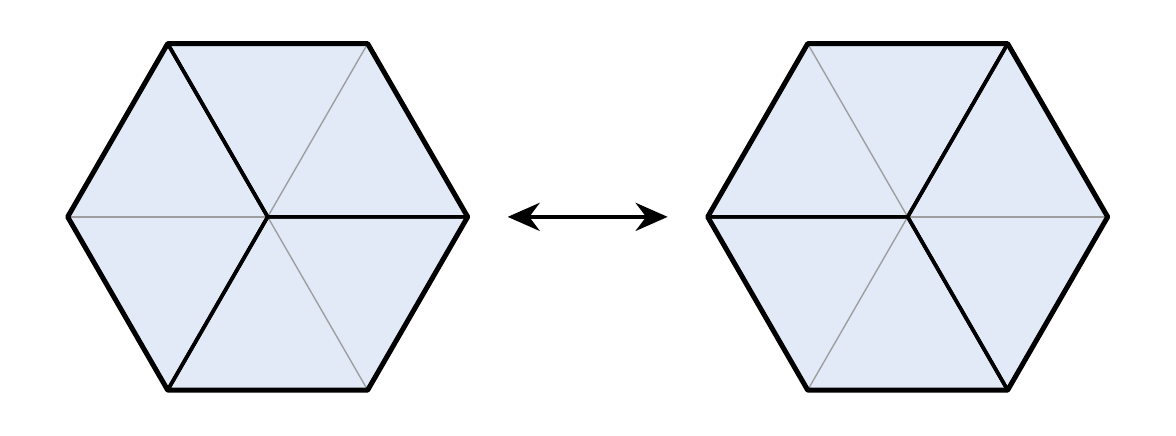
\begin{tikzpicture}[x=1in,y=1in]
\useasboundingbox (0,0) rectangle (5.6,-1.9);
\fill[white] (0.2,-0.946) -- (0.7,-1.8121) -- (1.7,-1.8121) -- (2.2,-0.946) -- (1.7,-0.08) -- (0.7,-0.08) -- cycle;
\fill[rhfill] (0.7,-1.8121) -- (1.2,-0.946) -- (0.7,-0.08) -- (0.2,-0.946) -- cycle;
\fill[rhfill] (0.7,-1.8121) -- (1.7,-1.8121) -- (2.2,-0.946) -- (1.2,-0.946) -- cycle;
\fill[rhfill] (1.2,-0.946) -- (2.2,-0.946) -- (1.7,-0.08) -- (0.7,-0.08) -- cycle;
\draw[gridline] (0.2,-0.946) -- (1.2,-0.946);
\draw[gridline] (0.7,-0.08) -- (1.2,-0.946);
\draw[gridline] (0.7,-1.8121) -- (1.2,-0.946);
\draw[gridline] (1.2,-0.946) -- (1.7,-0.08);
\draw[gridline] (1.2,-0.946) -- (1.7,-1.8121);
\draw[gridline] (1.2,-0.946) -- (2.2,-0.946);
\draw[line width=1.3pt, line join=round] (0.7,-1.8121) -- (1.2,-0.946) -- (0.7,-0.08) -- (0.2,-0.946) -- cycle;
\draw[line width=1.3pt, line join=round] (0.7,-1.8121) -- (1.7,-1.8121) -- (2.2,-0.946) -- (1.2,-0.946) -- cycle;
\draw[line width=1.3pt, line join=round] (1.2,-0.946) -- (2.2,-0.946) -- (1.7,-0.08) -- (0.7,-0.08) -- cycle;
\draw[line width=1.8pt, line join=round] (0.2,-0.946) -- (0.7,-1.8121) -- (1.7,-1.8121) -- (2.2,-0.946) -- (1.7,-0.08) -- (0.7,-0.08) -- cycle;
\draw[{Stealth[length=0.16in, width=0.14in]}-{Stealth[length=0.16in, width=0.14in]}, line width=1.6pt] (2.4,-0.946) -- (3.2,-0.946);
\fill[white] (3.4,-0.946) -- (3.9,-1.8121) -- (4.9,-1.8121) -- (5.4,-0.946) -- (4.9,-0.08) -- (3.9,-0.08) -- cycle;
\fill[rhfill] (3.9,-1.8121) -- (4.9,-1.8121) -- (4.4,-0.946) -- (3.4,-0.946) -- cycle;
\fill[rhfill] (3.4,-0.946) -- (4.4,-0.946) -- (4.9,-0.08) -- (3.9,-0.08) -- cycle;
\fill[rhfill] (4.9,-1.8121) -- (5.4,-0.946) -- (4.9,-0.08) -- (4.4,-0.946) -- cycle;
\draw[gridline] (3.4,-0.946) -- (4.4,-0.946);
\draw[gridline] (3.9,-0.08) -- (4.4,-0.946);
\draw[gridline] (3.9,-1.8121) -- (4.4,-0.946);
\draw[gridline] (4.4,-0.946) -- (4.9,-0.08);
\draw[gridline] (4.4,-0.946) -- (4.9,-1.8121);
\draw[gridline] (4.4,-0.946) -- (5.4,-0.946);
\draw[line width=1.3pt, line join=round] (3.9,-1.8121) -- (4.9,-1.8121) -- (4.4,-0.946) -- (3.4,-0.946) -- cycle;
\draw[line width=1.3pt, line join=round] (3.4,-0.946) -- (4.4,-0.946) -- (4.9,-0.08) -- (3.9,-0.08) -- cycle;
\draw[line width=1.3pt, line join=round] (4.9,-1.8121) -- (5.4,-0.946) -- (4.9,-0.08) -- (4.4,-0.946) -- cycle;
\draw[line width=1.8pt, line join=round] (3.4,-0.946) -- (3.9,-1.8121) -- (4.9,-1.8121) -- (5.4,-0.946) -- (4.9,-0.08) -- (3.9,-0.08) -- cycle;
\end{tikzpicture}
\par}
\vspace{0.12in}

Give your six ways of covering hexagon C the numbers 1 to 6. Make a map: draw a dot for each way, and draw a line between two dots when one flip changes one way into the other. Which two ways need the most flips to get from one to the other, and how many flips do they need?

\vspace{0.12in}
\fig{g45-p2}

\newpage
\withpic{4.15in}{\problem{3} In any covering of a hexagon whose bottom edge is one small edge long, the rhombus sitting on the bottom edge lies flat, so its top edge is flat too. The rhombus sitting on that edge also lies flat, and so on up to the top edge of the hexagon. These rhombuses form a chain. Write R for each rhombus in the chain that leans right and L for each one that leans left, from the bottom up. In the picture the chain is shaded, and its letters are R~L~R~R.}{g45-chain-example}

\vspace{0.15in}
Write the chain letters for each of your six ways of covering hexagon C. Could two different ways of covering hexagon C have the same chain letters? Explain. What happens to the chain letters when you make one flip?

\vspace{0.05in}
\fig{g45-p3}

\newpage
\problem{4} How many ways are there to cover each of these hexagons with blue rhombuses? Explain how you know each count is right.

\vspace{0.1in}
\fig{g45-p4d}

\newpage
\fig{g45-p4e}

\newpage
\fig{g45-p4f}

\newpage
\withpic{4.75in}{\problem{5} Each board below has a start covering printed on it. Build it with blue rhombuses. Then, using only flips, change it into the finish picture beside it, with as few flips as you can. Name each flip by the number of the point at its center, as in the small numbered hexagon. Write the points you flipped, in order, and the number of flips. For board c, explain why nobody can do it in fewer flips.}{g45-key}

\vspace{0.1in}
\fig{g45-p5a}

\newpage
{\raggedleft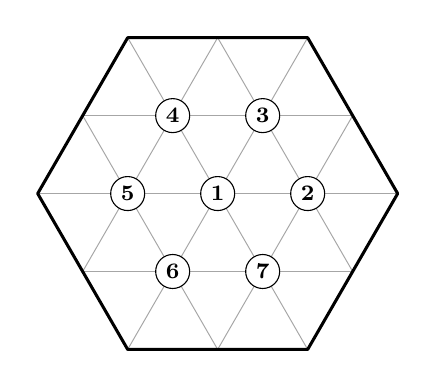
\begin{tikzpicture}[x=1in,y=1in]
\useasboundingbox (0,0) rectangle (1.9,-1.6588);
\fill[white] (0.5,-1.6088) -- (1.4,-1.6088) -- (1.85,-0.8294) -- (1.4,-0.05) -- (0.5,-0.05) -- (0.05,-0.8294) -- cycle;
\draw[gridsmall] (0.05,-0.8294) -- (0.5,-0.8294);
\draw[gridsmall] (0.275,-0.4397) -- (0.5,-0.8294);
\draw[gridsmall] (0.275,-0.4397) -- (0.725,-0.4397);
\draw[gridsmall] (0.5,-0.05) -- (0.725,-0.4397);
\draw[gridsmall] (0.275,-1.2191) -- (0.5,-0.8294);
\draw[gridsmall] (0.275,-1.2191) -- (0.725,-1.2191);
\draw[gridsmall] (0.5,-0.8294) -- (0.725,-0.4397);
\draw[gridsmall] (0.5,-0.8294) -- (0.725,-1.2191);
\draw[gridsmall] (0.5,-0.8294) -- (0.95,-0.8294);
\draw[gridsmall] (0.725,-0.4397) -- (0.95,-0.05);
\draw[gridsmall] (0.725,-0.4397) -- (0.95,-0.8294);
\draw[gridsmall] (0.725,-0.4397) -- (1.175,-0.4397);
\draw[gridsmall] (0.95,-0.05) -- (1.175,-0.4397);
\draw[gridsmall] (0.5,-1.6088) -- (0.725,-1.2191);
\draw[gridsmall] (0.725,-1.2191) -- (0.95,-0.8294);
\draw[gridsmall] (0.725,-1.2191) -- (0.95,-1.6088);
\draw[gridsmall] (0.725,-1.2191) -- (1.175,-1.2191);
\draw[gridsmall] (0.95,-0.8294) -- (1.175,-0.4397);
\draw[gridsmall] (0.95,-0.8294) -- (1.175,-1.2191);
\draw[gridsmall] (0.95,-0.8294) -- (1.4,-0.8294);
\draw[gridsmall] (1.175,-0.4397) -- (1.4,-0.05);
\draw[gridsmall] (1.175,-0.4397) -- (1.4,-0.8294);
\draw[gridsmall] (1.175,-0.4397) -- (1.625,-0.4397);
\draw[gridsmall] (0.95,-1.6088) -- (1.175,-1.2191);
\draw[gridsmall] (1.175,-1.2191) -- (1.4,-0.8294);
\draw[gridsmall] (1.175,-1.2191) -- (1.4,-1.6088);
\draw[gridsmall] (1.175,-1.2191) -- (1.625,-1.2191);
\draw[gridsmall] (1.4,-0.8294) -- (1.625,-0.4397);
\draw[gridsmall] (1.4,-0.8294) -- (1.625,-1.2191);
\draw[gridsmall] (1.4,-0.8294) -- (1.85,-0.8294);
\draw[line width=1.1pt, line join=round] (0.5,-1.6088) -- (1.4,-1.6088) -- (1.85,-0.8294) -- (1.4,-0.05) -- (0.5,-0.05) -- (0.05,-0.8294) -- cycle;
\node[circle, draw, fill=white, inner sep=0.6pt, minimum size=0.17in, font=\footnotesize\bfseries] at (0.95,-0.8294) {1};
\node[circle, draw, fill=white, inner sep=0.6pt, minimum size=0.17in, font=\footnotesize\bfseries] at (1.4,-0.8294) {2};
\node[circle, draw, fill=white, inner sep=0.6pt, minimum size=0.17in, font=\footnotesize\bfseries] at (1.175,-0.4397) {3};
\node[circle, draw, fill=white, inner sep=0.6pt, minimum size=0.17in, font=\footnotesize\bfseries] at (0.725,-0.4397) {4};
\node[circle, draw, fill=white, inner sep=0.6pt, minimum size=0.17in, font=\footnotesize\bfseries] at (0.5,-0.8294) {5};
\node[circle, draw, fill=white, inner sep=0.6pt, minimum size=0.17in, font=\footnotesize\bfseries] at (0.725,-1.2191) {6};
\node[circle, draw, fill=white, inner sep=0.6pt, minimum size=0.17in, font=\footnotesize\bfseries] at (1.175,-1.2191) {7};
\end{tikzpicture}
\par}
\vspace{0.05in}
\fig{g45-p5b}

\newpage
\withpic{4.75in}{\problem{6} Start from the covering printed on the board. A round trip is a list of flips that brings the board back exactly to the start. Find a round trip of 4 flips and a round trip of 6 flips that never flip at the same point twice in a row. Write the points in order, using the numbers in the small hexagon. Can a round trip have an odd number of flips, such as 3, 5 or 7? Explain.}{g45-key}

\vspace{0.15in}
\fig{g45-p6}

\newpage
\problem{7} How many ways are there to cover this hexagon with blue rhombuses? Explain how you know you have found them all.

\vspace{0.1in}
\fig{g45-p7}

\end{document}
